\documentclass[xcolor=dvipsnames,t]{beamer} % position stuff on top of slide
% Functions, packages, etc.
%[[[
\usetheme{Frankfurt}
\usecolortheme[named=Maroon]{structure}

% Remove Navigation Symbols
\usenavigationsymbolstemplate{}

\usepackage{mathdots} % for \iddots

\usepackage{tikz}
\usetikzlibrary{matrix}
\usetikzlibrary{calc}
\tikzset{node style ge/.style={circle}}

\usepackage{amsmath}
\usepackage{amsfonts}
\usepackage{amssymb}
\usepackage{amsthm}
\usepackage{array}

\usepackage{tikz,gnuplot-lua-tikz}
%\usetikzlibrary{external} % speed up TikZ compilation by caching figures; use lualatex over pdflatex (dynamic memory alloc)
%%XXX need to add -enable-write18 to initial lualatex call in Makefile
%\tikzexternalize[prefix=tikz_cache/]
%\tikzset{external/system call={lualatex
%      \tikzexternalcheckshellescape -halt-on-error -interaction=batchmode
%-jobname "\image" "\texsource"}}%

\usepackage{graphicx}
%\usepackage{subfig}
\usepackage[labelfont=bf]{caption}
%\usepackage[labelfont=bf]{subcaption}
%\usepackage[top=1in, bottom=1in, left=1in, right=1in]{geometry}
%\pagenumbering{arabic}
\usepackage{hyperref}
%\numberwithin{equation}{section}
%\usepackage{soul} % for \ul - a ``better'' underlining command

%\usepackage{colortbl} % for coloring \multicolumn (tabular in general, I think)
% For \rowcolor
%\definecolor{table_header}{gray}{0.5}
%\definecolor{table_data}{gray}{0.85}

\usepackage{algorithm}
\usepackage{algpseudocode,algorithmicx}

%% Inserting code and syntax highlighting
%% [[[
%\usepackage{listings} % like verbatim, but allows for syntax highlighting and more
%\usepackage{color} % colors
%\usepackage[usenames,dvipsnames]{xcolor}% More colors
%\usepackage{caption} % captions
%\DeclareCaptionFont{white}{\color{white}}
%\DeclareCaptionFormat{listing}{\colorbox{gray}{\parbox{\textwidth}{#1#2#3}}}
%\captionsetup[lstlisting]{format=listing,labelfont=white,textfont=white}
%\usepackage{framed} % put a frame around things
%
%% define some custom colors
%\definecolor{dkgreen}{rgb}{0,0.6,0}
%\definecolor{lgreen}{rgb}{0.25,1,0}
%\definecolor{purple}{rgb}{0.35,0.02,0.48}
%
%% Some changes to MATLAB/GNU Octave language in listings
%\lstset{frame=tbrl,
%    language=Matlab,
%    aboveskip=3mm,
%    belowskip=3mm,
%    belowcaptionskip=3mm,
%    showstringspaces=false,
%    columns=flexible,
%    basicstyle={\small\ttfamily\color{black}},
%    numbers=left,
%    numberstyle=\tiny\color{purple},
%    keywordstyle=\color{dkgreen},
%    commentstyle=\color{red},
%    stringstyle=\color{purple},
%    breaklines=true,
%    breakatwhitespace=true,
%    tabsize=4,
%    rulecolor=\color{black},
%    morekeywords={string,fstream}
%}
%% ]]]


%My Functions
\newcommand{\diff}[2]{\dfrac{d #1}{d #2}}
\newcommand{\diffn}[3]{\dfrac{d^{#3} #1}{d {#2}^{#3}}}
\newcommand{\pdiff}[2]{\dfrac{\partial #1}{\partial #2}}
\newcommand{\pdiffn}[3]{\dfrac{\partial^{#3} #1}{\partial {#2}^{#3}}}
\newcommand{\problemline}{\rule{\textwidth}{0.25mm}}
%\newcommand{\problem}[1]{\problemline\\#1\\\problemline\vspace{10pt}}
\newcommand{\reals}{\mathbb{R}}
\newcommand{\qline}[2]{\qbezier(#1)(#1)(#2)}
\newcommand{\abox}[1]{\begin{center}\fbox{#1}\end{center}}
\newcommand{\lie}{\mathcal{L}}
%\newcommand{\defeq}{\stackrel{\operatorname{def}}{=}}

% AMS theorem stuff
%% [[[
%\newtheoremstyle{mystuff}{}{}{\itshape}{}{\bfseries}{:}{.5em}{}
%\theoremstyle{mystuff}
%\newtheorem{definition}{Definition}[section]
%\newtheorem*{definition*}{Definition}
%\newtheorem{theorem}{Theorem}[section]
%\newtheorem*{theorem*}{Theorem}
%\newtheorem{lemma}{Lemma}[section]
%\newtheorem*{lemma*}{Lemma}
%\newtheorem{proposition}{Proposition}[section]
%\newtheorem*{proposition*}{Proposition}
%\newtheorem*{corollary*}{Corollary}
%\newtheorem*{remark}{Remark}
%
%\newtheoremstyle{myexample}{}{}{}{}{\bfseries}{:}{.5em}{}
%\theoremstyle{myexample}
%\newtheorem*{example*}{Example}
%
%% Stolen from http://tex.stackexchange.com/questions/8089/changing-style-of-proof
%\makeatletter \renewenvironment{proof}[1][\proofname] {\par\pushQED{\qed}\itshape\topsep6\p@\@plus6\p@\relax\trivlist\item[\hskip\labelsep\bfseries#1\@addpunct{:}]\ignorespaces}{\popQED\endtrivlist\@endpefalse} \makeatother
%
%% Stolen from http://tex.stackexchange.com/questions/12913/customizing-theorem-name
%\newtheoremstyle{named}{}{}{\itshape}{}{\bfseries}{:}{.5em}{\thmnote{#3's }#1}
%\theoremstyle{named}
%\newtheorem*{namedtheorem}{Theorem}
%% ]]]

%]]]


% Output Control Variables
\def\true{1}
\def\false{0}
\def\figures{1}
\def\tables{1}

\renewcommand{\UrlFont}{\scriptsize}
\newcommand{\defeq}{\mathrel{\mathop:}=}
\DeclareMathOperator*{\argmin}{arg\,min}

% http://tex.stackexchange.com/questions/43065/matrices-too-big-to-fit-the-width-of-a-page
\newcommand\scalemath[2]{\scalebox{#1}{\mbox{\ensuremath{\displaystyle #2}}}}

\title{Application of Adjoint Operators in Gradient Computations}
\date{5 March, 2016}
\author{James Folberth\\Advisor: Stephen Becker}
\institute{University of Colorado at Boulder}

\begin{document}

\begin{frame}
\maketitle
\end{frame}

\begin{frame}{Outline}
   \begin{enumerate}
      \item A model optimiztion problem
      \item Example 1: Image Deblurring
      \item Example 2: Blind Channel Estimation
   \end{enumerate}

   %TODO put in a blurred image -> deblurred image to fill space?

\end{frame}

\section{Model Problem}
% [[[
\begin{frame}{A Model Problem}
   Consider

   \[ \min_x \dfrac{1}{2}\|\mathcal{A}x-b\|_2^2 + \lambda \|x\|_1. \] 

   \begin{itemize}
      \item $\mathcal{A}$ is a linear operator on problem variable $x$.
      \item $b$ is measured data (e.g. blurry image).
      \item Include $\lambda \|x\|_1$, to induce sparsity in $x$ (hopefully).
   \end{itemize}

   Define 

   \[ f(x) = \dfrac{1}{2}\|\mathcal{A}x-b\|_2^2, \quad g(x) = \lambda \|x\|_1. \] 

   \noindent $f(x)$ is convex, differentiable, $g(x)$ is convex, non-differentiable.
   
   \[ \nabla f(x) = \mathcal{A}^\ast\left(\mathcal{A}x-b\right). \] 

\end{frame}

\begin{frame}{Proximal Gradient Method}
   \[ f(x) = \dfrac{1}{2}\|\mathcal{A}x-b\|_2^2, \quad g(x) = \lambda \|x\|_1. \] 

   We can use a variant of simple gradient descent to solve the model problem

   \[ \min_x f(x) + g(x). \] 

   %XXX dropping k step notation for brevity.  x^+ is the new x after the prox grad step
   Proximal gradient method:
   \[ x^{+} = \operatorname{prox}_{t g}\left(x - t\nabla f(x)\right), \text{ step size $t>0$}. \] 
   
   Proximity function: 
   \[ \operatorname{prox}_g(x) \defeq \argmin_u\left(g(u) + \dfrac{1}{2}\|u-x\|_2^2\right). \] 

\end{frame}

\begin{frame}{Proximal Gradient Method}
   %\[ x^{(k)} = \operatorname{prox}_{t_k g}\left(x^{(k-1)} - t_k\nabla f(x^{(k-1)})\right). \] 
   \[ \operatorname{prox}_g(x) \defeq \argmin_u\left(g(u) + \dfrac{1}{2}\|u-x\|_2^2\right). \] 

   For $g(x) = \lambda\|x\|_1$, proximity operator is ``shrinkage'':

   \[ \left\{\operatorname{prox}_g(x)\right\}_i = \left\{\begin{array}{ll} x_i-\lambda & x_i \ge \lambda\\0 & |x_i| < \lambda\\ x_i + \lambda & x_i\le -\lambda\end{array}\right.. \] 

   %XXX dropping k step notation for brevity.  x^+ is the new x after the prox grad step
   Proximal gradient step minimizes $g(u)$ plus quadratic local model of $f(u)$ about $x$:

   \begin{align*}
      x^+ &= \operatorname{prox}_{t g}\left(x - t\nabla f(x)\right)\\
              %&= \argmin_u\left(g(u) + \dfrac{1}{2t}\left\|u-x+t\nabla f(x)\right\|_2^2\right)\\
              &= \argmin_u\left(g(u) + f(x) + \left\langle \nabla f(x), u-x\right\rangle + \dfrac{1}{2t}\|u-x\|_2^2\right).
   \end{align*}

\end{frame}

\begin{frame}{Proximal Gradient Method}
   \[ \min_x \dfrac{1}{2}\|\mathcal{A}x-b\|_2^2 + \lambda \|x\|_1. \] 

   \[ \nabla f(x) = \mathcal{A}^\ast\left(\mathcal{A}x-b\right), \quad x^{+} = \operatorname{prox}_{t g}\left(x - t\nabla f(x)\right)\] 

   \noindent Need to efficiently compute
   \begin{itemize}
      \item $\operatorname{prox}_{tg}(x)$ with $g(x) = \lambda \|x\|_1$.  ``Shrinkage'' is fast.
      \item $\mathcal{A}$.  Usually have fast forward and inverse transform (e.g. FFT, discrete wavelet transform).
      \item $\mathcal{A}^\ast$.  Sometimes not so easy...  Let's look at a couple examples.
   \end{itemize}
\end{frame}

% ]]]


\section{Image Deblurring}
% [[[
\begin{frame}{Image Deblurring Problem}
   Observation: natural images tend to have sparse wavelet coefficients.\\
   
   \begin{itemize}
      \item $b$ - observed blurred image, with known blurring operator $\mathcal{R}$\\ (e.g. Gaussian PSF applied efficiently in Fourier domain)
      \item $\mathcal{W}$ - multi-level wavelet synthesis operator
      \item $x$ - wavelet coefficients
   \end{itemize}

   Natural problem formulation is

   \[ \min_x \dfrac{1}{2}\left\|\mathcal{RW}x-b\right\|_2^2 + \lambda \|x\|_1. \]

   \[ \nabla f(x) = \mathcal{W}^\ast\mathcal{R}^\ast\left(\mathcal{RW}x-b\right). \] 

\end{frame}

\begin{frame}{Image Deblurring Problem}
   \begin{center}
   \begin{columns}[t]
      \begin{column}{0.45\textwidth}
         Observed image:
         \includegraphics[width=\textwidth]{../ieee_spm/figures/cameraman_observed_trim.pdf}
      \end{column}
      
      \begin{column}{0.45\textwidth}
         Recovered image:
         \includegraphics[width=\textwidth]{../ieee_spm/figures/{cameraman_rec_200_bior4.4_sym_trim}.pdf}
      \end{column}
   \end{columns}
   \end{center}
\end{frame}

\begin{frame}{Adjoint of Wavelet Operator}
   \[ \nabla f(x) = \mathcal{W}^\ast\mathcal{R}^\ast\left(\mathcal{RW}x-b\right). \] 
   
   \begin{itemize}
      \item $\mathcal{W}$ is wavelet synthesis (reconstruction).  Standard routine in libraries.
      % actually DCT is used for symmetric/reflexive BCs
      \item $\mathcal{R}$ and $\mathcal{R}^\ast$ for blurring PSF can be applied rapidly in Fourier domain (FFT).
      \item What about $\mathcal{W}^\ast$?  Not a standard operation like $\mathcal{W}$ and $\mathcal{W}^\dagger$.
   \end{itemize}

   If $\mathcal{W}$ is orthogonal, $\mathcal{W}^\ast = \mathcal{W}^\dagger$.\\
   If $\mathcal{W}$ is biorthogonal, $\mathcal{W}^\ast \approx \mathcal{W}^\dagger$.\\
   So, one option is

   \[ \nabla f(x) \approx \mathcal{W}^\dagger\mathcal{R}^\ast\left(\mathcal{RW}x-b\right). \]
   
   % And many people use this approach.  It actually works pretty well.  But how much error does W^* = W^+ indtroduct?
\end{frame}

\begin{frame}{Adjoint of Wavelet Operator}
   We could use $\mathcal{W}^\ast \approx \mathcal{W}^\dagger$, but it turns out we can find the adjoint exactly!\\
   
   \begin{itemize}
      \item Related to $\mathcal{W}$ are frame vectors $\phi_n$ (the wavelet basis vectors), which define a frame operator $\Phi=\mathcal{W}^\dagger$:

         \[ \Phi f[n] = \langle f, \phi_n\rangle. \] 
      \item We can define the dual frame vectors $\tilde{\phi}_n=\left(\Phi^\ast\Phi\right)^{-1}\phi_n$.
      \item Define the dual frame operator via

         \[ \tilde{\Phi}f[n] = \langle f, \tilde{\phi}_n\rangle. \] 

      \item Digging around in frame theory a bit, we find

         \[ \Phi^\ast = \tilde{\Phi}^\dagger \implies {\color{blue}\mathcal{W}^\ast = \tilde{\mathcal{W}}^\dagger}\] 
   \end{itemize}

\end{frame}

\begin{frame}{Adjoint of Wavelet Operator}
   So we have $\mathcal{W}^\ast = \tilde{\mathcal{W}}^\dagger$: the adjoint of wavelet synthesis is dual wavelet reconstruction.\\

   But we must also handle boundary conditions.\\

   This is usually done by extending the signal via $\mathcal{E}$ to satisfy the BCs.\\

   The relation $\mathcal{W}^\ast = \tilde{\mathcal{W}}^\dagger$ holds for $\mathcal{E}$ being zero-padding, since $\mathcal{E}^\ast = \mathcal{E}^\dagger$.  Let $\mathcal{W}_\text{zpd}$ be wavelet synthesis with zero BCs.\\

   In general, we have

   \[ \mathcal{W}^\dagger = \mathcal{W}_\text{zpd}^\dagger\mathcal{E} \implies \mathcal{W}=\mathcal{E}^\dagger\mathcal{W}_\text{zpd} \implies \mathcal{W}^\ast = \mathcal{W}_\text{zpd}^\ast\left(\mathcal{E}^\dagger\right)^\ast \]

   and

   \[ {\color{blue} \mathcal{W}^\ast = \tilde{\mathcal{W}}_\text{zpd}^\dagger \left(\mathcal{E}^\dagger\right)^\ast}. \] 


\end{frame}

\begin{frame}{Adjoint of Extension Pseudoinverse}
   Due to factorization $\mathcal{W}^\ast = \tilde{\mathcal{W}}_\text{zpd}^\dagger(\mathcal{E}^\dagger)^\ast$, we just need to implement $(\mathcal{E}^\dagger)^\ast$!  $\tilde{\mathcal{W}}_\text{zpd}^\dagger$ is a standard and fast operation.\\[.5em]

   Consider a signal $y[n]$, $n=0,...,N-1$.  Let $L_p$ be the length of wavelet analysis filters.\\[.5em]

   Zero padding:
   \[ \underbrace{0, ..., 0}_{L_p-1}, y[0], ..., y[N-1], \underbrace{0, ..., 0}_{L_p-1}. \]

   Half-point symmetric:
   \[ \underbrace{y[L_p-1], ..., y[0]}_\text{Left extension}, y[0], ..., y[N-1], \underbrace{y[N-1], ..., y[N+L_p-2]}_\text{Right extension}. \] 

\end{frame}

\begin{frame}{Zero padding}
   Zero padding as a linear operator:

   \begin{columns}
      \begin{column}{0.7\textwidth}
\[ \mathcal{E}_\text{zpd} = \begin{bmatrix} 0_{(L_p-1)\times N}\\ I_{N\times N}\\ 0_{(L_p-1)\times N}\end{bmatrix} = \begin{bmatrix} 0 & 0 & \cdots & 0 & 0\\ \vdots & \vdots &\ddots & \vdots & \vdots\\ 0 & 0 & \cdots & 0 & 0\\[0.5em] 1 & 0 & \cdots & 0 & 0\\ 0 & 1 & \cdots & 0 & 0\\ \vdots & \vdots & \ddots & \vdots & \vdots\\ 0 & 0 & \cdots & 1 & 0\\ 0 & 0 & \cdots & 0 & 1\\[0.5em] 0 & 0 & \cdots & 0 & 0\\ \vdots & \vdots & \ddots & \vdots & \vdots\\ 0 & 0 & \cdots & 0 & 0\end{bmatrix}. \] 
      \end{column}

      \begin{column}{0.3\textwidth}
         In this case

         \[ \left(\mathcal{E}_\text{zpd}^\dagger\right)^\ast = \mathcal{E}_\text{zpd}. \] 

         \noindent This is what allows us the factorization

         \[ \mathcal{W}^\ast = \tilde{\mathcal{W}}_\text{zpd}^\dagger \left(\mathcal{E}^\dagger\right)^\ast. \] 


      \end{column}
   \end{columns}
\end{frame}

\begin{frame}{Half-point symmetric}
   Half-point symmetric extension as a linear operator:

\[ \scalemath{0.75}{\mathcal{E}_\text{sym} = \begin{bmatrix} & & \iddots & & &\\ & 1 &&&&\\ 1&&&&&\\1&&&&\\&1&&&&\\&&\ddots&&&\\&&&1&\\&&&&1\\&&&&1\\&&&1&\\&&\iddots&&\end{bmatrix}, \quad \left(\mathcal{E}_\text{sym}^\dagger\right)^\ast = \scalemath{0.75}{\begin{bmatrix} & \iddots \\ 1/2&&&&&\\1/2&&&&\\&\ddots&&&&&&\\&&1/2&\\&&&1\\&&&&\ddots\\&&&&&1\\&&&&&&1/2\\&&&&&&&\ddots\\&&&&&&&&1/2\\&&&&&&&&1/2\\&&&&&&&\iddots\\\end{bmatrix}}}. \]

\end{frame}

\begin{frame}{Image Deblurring Problem}
   \begin{itemize}
      \item $\mathcal{W}^\ast = \tilde{\mathcal{W}}_\text{zpd}^\dagger(\mathcal{E}^\dagger)^\ast$.
      \item $\tilde{\mathcal{W}}^\dagger$ is part of wavelet library and is fast.
      \item $(\mathcal{E}^\dagger)^\ast$ is closed-form and fast.
      \item So we can apply $\mathcal{W}^\ast$ efficiently in

         \[ \nabla f(x) = \mathcal{W}^\ast\mathcal{R}^\ast\left(\mathcal{RW}x-b\right). \] 
   \end{itemize}
\end{frame}

\begin{frame}{Image Deblurring Problem}
   $200$ iterations of FISTA, $\mathcal{W}^\dagger$ is a 3-stage CDF 9/7 wavelet transform, ${\lambda = 2\times 10^{-5}}$
   \begin{center}
   \begin{columns}[t]
      \begin{column}{0.45\textwidth}
         Using $\mathcal{W}^\ast \approx \mathcal{W}^\dagger$:
         \includegraphics[width=\textwidth]{../ieee_spm/figures/{cameraman_rec_200_bior4.4_sym_badjoint_trim}.pdf}

         \[ \scalemath{0.75}{\dfrac{\|\mathcal{W}x-y\|_2}{\|y\|_2} = 7.25\times 10^{-2}} \] 
      \end{column}
      
      \begin{column}{0.45\textwidth}
         Using $\mathcal{W}^\ast = \tilde{\mathcal{W}}_\text{zpd}^\dagger(\mathcal{E}^\dagger)^\ast$:
         \includegraphics[width=\textwidth]{../ieee_spm/figures/{cameraman_rec_200_bior4.4_sym_trim}.pdf}
         \[ \scalemath{0.75}{\dfrac{\|\mathcal{W}x-y\|_2}{\|y\|_2} = 7.24\times 10^{-2}} \] 
      \end{column}
   \end{columns}
   \end{center}

\end{frame}

% ]]]


\section{Blind Channel Estimation}
% [[[
\begin{frame}{BCE Problem}
   Unknown source $s$ sends signal over unknown channels with impulse response $h_i$.  We observe channel outputs

   \[ x_i[n] = \{h_i\ast s\}[n]. \] 
   
   \noindent Can we recover source and channel IRs?\\

\end{frame}

\begin{frame}{BCE Problem}
   For simplicity of notation, consider a single channel $h$ with output $x$.  Let $h$ be of length $K$ and $s$ be of length $N$; $x$ will be of length $K+N-1$.\\[0.5em]

   One can write the convolution as linear operator on the $K\times N$ matrix $hs^T$:

   \[ x = h\ast s = \mathcal{A}(hs^T). \] 

   \noindent Assuming $h$ and $s$ should be sparse in time, a natural problem formulation is
      
   \[ \min_{h,s} \dfrac{1}{2}\|\mathcal{A}(hs^T)-x\|_2^2 + \lambda_h\|h\|_1 + \lambda_s\|s\|_1. \] 

   \noindent This is non-convex.  Can use other regularization terms (e.g. $\|h\|_\text{TV}$).
\end{frame}

\begin{frame}{Adjoint of $\mathcal{A}$}
   Define $f(h,s) = 1/2\|\mathcal{A}(hs^T)-x\|_2^2$.\\[.5em]
   
   The required gradients are
   \begin{align*}
      \nabla_h f(h,s) &= \left[\mathcal{A}^\ast(\mathcal{A}(hs^T)-x)\right]s\\
      \nabla_s f(h,s) &= \left[\mathcal{A}^\ast(\mathcal{A}(hs^T)-x)\right]^Th.
   \end{align*}

   Note that $\mathcal{A}$ takes a matrix and returns a vector.  So $\mathcal{A}^\ast$ must take a vector and return a matrix (of appropriate size).\\

\end{frame}

\begin{frame}{Adjoint of $\mathcal{A}$}
   We know the action of $\mathcal{A}(hs^T)$:
      
   \[ x[n] =  \sum_{k=k_1(n)}^{k_2(n)} h[k]s[n-k], \] 

   where $k_1(n) = \max\{0,n+1-N\}$ and $k_2(n) = \min\{K-1,n\}$.

\end{frame}

\begin{frame}{Adjoint of $\mathcal{A}$}
   We know the action of $\mathcal{A}(hs^T)$:

   \begin{center}
   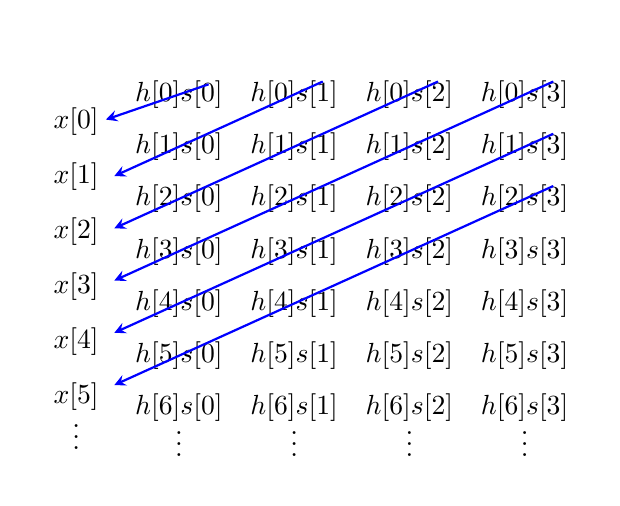
\begin{tikzpicture}[baseline=(hs.center), ampersand replacement=\&]
      % [[[
      % based on figure from Romberg et al. "Multichannel blind deconvolution..."
      % and examples from http://www.texample.net/tikz/examples/mnemonic-rule-for-matrix-determinant/
      % http://tex.stackexchange.com/questions/83046/position-two-stacked-tikz-matrices
      % http://www.texample.net/tikz/examples/energy-level-diagram/
      \matrix (hs) [matrix of math nodes, nodes = {node style ge},, column sep=0mm, row sep=-8mm]
      {h[0]s[0] \& h[0]s[1] \& h[0]s[2] \& h[0]s[3] \\
       h[1]s[0] \& h[1]s[1] \& h[1]s[2] \& h[1]s[3] \\
       h[2]s[0] \& h[2]s[1] \& h[2]s[2] \& h[2]s[3] \\
       h[3]s[0] \& h[3]s[1] \& h[3]s[2] \& h[3]s[3] \\
       h[4]s[0] \& h[4]s[1] \& h[4]s[2] \& h[4]s[3] \\
       h[5]s[0] \& h[5]s[1] \& h[5]s[2] \& h[5]s[3] \\
       h[6]s[0] \& h[6]s[1] \& h[6]s[2] \& h[6]s[3] \\
       \vdots \& \vdots \& \vdots \& \vdots\\
      };
   
      \begin{scope}[xshift=-35mm,yshift=-2.5mm]
      \matrix (y) [matrix of math nodes, nodes = {node style ge},, column sep=0mm, row sep=-3mm]
      {x[0]\\
       x[1]\\
       x[2]\\
       x[3]\\
       x[4]\\
       x[5]\\[-2mm]
       \vdots\\
      };
      \end{scope}
   
      \draw [thick,->,>=stealth,shorten >=4mm,shorten <=-4mm,color=blue] (hs-1-1.center) to ($(y-1-1.center) + (0mm,-1mm)$); % this is a hack, but it's quite close
      \draw [thick,->,>=stealth,shorten >=-9mm,shorten <=-4mm,color=blue] (hs-1-2.center) to (hs-2-1.center);
      \draw [thick,->,>=stealth,shorten >=-9mm,shorten <=-4mm,color=blue] (hs-1-3.center) to (hs-3-1.center);
      \draw [thick,->,>=stealth,shorten >=-9mm,shorten <=-4mm,color=blue] (hs-1-4.center) to (hs-4-1.center);
      \draw [thick,->,>=stealth,shorten >=-9mm,shorten <=-4mm,color=blue] (hs-2-4.center) to (hs-5-1.center);
      \draw [thick,->,>=stealth,shorten >=-9mm,shorten <=-4mm,color=blue] (hs-3-4.center) to (hs-6-1.center);
      % ]]]
   \end{tikzpicture}
   \end{center}

\end{frame}

%TODO show adjoint derivation (be brief!)
%TODO Hankel -> Toeplitz -> Circulant -> FFT!
%TODO show (stolen) picture of recovery

% ]]]

\begin{frame}{Thanks!}
   References:
\end{frame}

%\begin{frame}{Extra Slides}
%   %TODO might want to put prox grad details in here.
%   %TODO prox grad and FISTA side-by-side?
%   %TODO why not use analysis formulation of deblurring problem?
%   %TODO original cameraman and recovered image side-by-side
%\end{frame}

% [[[
%\begin{frame}{Ideas} Dr. Becker and I have been working on some ``warm-up'' problems this semester.  \begin{itemize} \item Can we use Nesterov accelerated gradient descent to train $K$-means or GMM's faster than the standard method?  \item The adjoint of a wavelet operator is required for some optimization problems, but is not provided by wavelet toolboxes.  Can we find a fast (e.g. $\mathcal{O}(N)$) way to compute its action?  \end{itemize} \end{frame} \section{$K$-means} \begin{frame}{$K$-means} \begin{figure}[ht!] \includegraphics[width=\textwidth]{figures/kmeans_22130988_true_labels_trim.pdf} \end{figure} \begin{itemize} \item $K$-means is a simple clustering algorithm.  True problem is NP hard, so we relax and find a local solution.  \end{itemize} \end{frame} \begin{frame}{$K$-means} \begin{figure}[ht!] \includegraphics[width=\textwidth]{figures/kmeans_22130988_hard_em!_trim.pdf} \end{figure} \begin{itemize} \item Initialization is very important (kmeans++ provides good error bounds) \end{itemize} \end{frame} \begin{frame}{$K$-means as a GMM} %$K$-means is a special case of a full Gaussian mixture model (GMM).\\ Cluster the data by maximizing the log-likelihood of the data: \[ \ell(\theta) = \sum_{n=1}^N \log\left(\sum_{k=1}^K \dfrac{1}{K}\mathcal{N}(\mathbf{x}_n|\mu_k,\sigma^2I)\right). \] \begin{columns} \begin{column}{0.5\textwidth} ``hard'' expectation maximization \[ z_i^\ast = \arg\min_k \|\mathbf{x}_i-\mu_k\|_2^2 \] \[ \mu_k \gets \dfrac{1}{N_k} \sum_{i:z_i=k} \mathbf{x}_i. \] 
%      \end{column}
%      \begin{column}{0.5\textwidth}
%         ``soft'' expectation maximization
%         \[ r_{ik} \propto e^{-\|\mathbf{x}_i-\mu_k\|_2^2/(2\sigma^2)}\] 
%         \[ z_i^\ast = \arg\max_k r_{ik} \] 
%         \[ \mu_k \gets \dfrac{1}{r_k}\sum_{i=1}^N r_{ik}\mathbf{x}_i, \quad r_k = \sum_{i=1}^N r_{ik}. \] 
%      \end{column}
%   \end{columns}
%
%\end{frame}
%
%\begin{frame}{$K$-means and gradient descent}
%   \begin{itemize}
%      \item Instead of expectation maximization (the standard algorithm), we could try to use gradient descent.\\
%
%      \item This works, and for a certain step size ($\eta_k = \sigma^2/r_k$), gradient descent is equivalent to expectation maximization.  GD is slow, taking $\mathcal{O}(1/\epsilon)$ iterations to reach suboptimality $\epsilon$.
%
%      \item Nesterov's accelerated gradient is optimal, in a certain sense, and takes $\mathcal{O}(1/\sqrt{\epsilon})$ iterations to reach suboptimality $\epsilon$, for certain problems.
%
%      \item The ``soft'' $K$-means problem is non-convex and doesn't have a Lipschitz gradient.  Existing convergence proofs don't apply.  Works well in practice, though!
%   \end{itemize}
%\end{frame}
%
%\begin{frame}{A Nesterov accelerated gradient method}
%   Nesterov acceleration is super cheap; basically the same cost as gradient descent.\\[1em]
%
%   \begin{algorithm}[H] % force it to stay in its place with `H'
%   \caption{Nesterov's second method}
%   \begin{algorithmic}
%      \State Given initial point $x^{(0)}$.
%      \State $v^{(0)}\gets x^{(0)}$
%      \For{k\ge 1}
%         \State $\theta^{(k)} = \frac{2}{k+1}$
%         \State $y\gets (1-\theta^{(k)})x^{(k-1)} + \theta^{(k)}v^{(k-1)}$
%         \State $v^{(k)} \gets v^{(k-1)} + \dfrac{\eta^{(k)}}{\theta^{(k)}}\nabla\ell(y)$
%         \State $x^{(k)} \gets (1-\theta^{(k)})x^{(k-1)} + \theta^{(k)}v^{(k)}$
%      \EndFor
%   \end{algorithmic}
%\end{algorithm}
%\end{frame}
%
%
%\begin{frame}{Performance profiles: $d=3, K=40, N=3000$}
%   \begin{figure}[ht!]
%      \includegraphics[width=\textwidth]{/home/james/research/mm_methods/accelerated_em/unwatched/n=3_K=40_N=3000_iter.pdf}
%   \end{figure}
%\end{frame}
%
%\begin{frame}{Performance profiles: $d=40, K=40, N=3000$}
%   \begin{figure}[ht!]
%      \includegraphics[width=\textwidth]{/home/james/research/mm_methods/accelerated_em/unwatched/n=40_K=40_N=3000_iter2.pdf}
%   \end{figure}
%\end{frame}
%
%\begin{frame}{Performance profiles: $d=40, K=40, N=3000$}
%   \begin{figure}[ht!]
%      \includegraphics[width=\textwidth]{/home/james/research/mm_methods/accelerated_em/unwatched/n=40_K=40_N=3000_time.pdf}
%   \end{figure}
%\end{frame}
%
%
%\section{Gaussian Mixture Models}
%\begin{frame}{Extend to GMMs?}
%   \begin{itemize}
%      \item We think we might be able to apply a Nesterov method to a full GMM.
%      \item Implementation and analysis is harder.
%      \item Performance might not be sufficiently better than EM.
%   \end{itemize}
%
%   \[ \ell(\theta) = \sum_{n=1}^N \log\left(\sum_{k=1}^K \pi_k \mathcal{N}(\mathbf{x}_n|\mu_k, \Sigma_k)\right). \] 
%\end{frame}
%
%
%\section{Wavelet-based Image Deblurring}
%\begin{frame}{Problem Statement}
%   We're given a blurred image $\tilde{x}$ and know more-or-less how it was distorted (e.g. point spread function (PSF)).\\
%
%   We want to find the original image.
%
%   \[ \begin{array}{ll} \text{min}_x & \|RW^\dagger x - \tilde{x}\|_2^2 + \lambda \|x\|_1 \end{array}. \] 
%
%   \begin{itemize}
%      \item $R$ - blurring operator; fast computation via FFT
%      \item $W^\dagger$ - (multi-level) wavelet synthesis operator
%      \item $x$ - wavelet coefficients (problem variable)
%      \item $\lambda$ - regularization parameter
%      \item $\|x\|_1$ - hopefully produces sparse coefficients $x$
%   \end{itemize}
%\end{frame}
%
%\begin{frame}{Adjoint Wavelet Operator}
%   Split the objective function
%   
%   \[ \begin{array}{ll} \text{min}_x & f(x) + g(x)\end{array}, \quad f(x) = \|RW^\dagger x - \tilde{x}\|_2^2, \quad g(x) = \lambda \|x\|_1. \] 
%
%   To solve with a fast proximal gradient method, we need $\nabla f(x)$, but not $\nabla g(x)$:
%
%   \[ \nabla f(x) = 2 (W^\dagger)^\ast R^\ast\left(RW^\dagger x-\tilde{x}\right). \] 
%   
%   \noindent Need to compute $(W^\dagger)^\ast$ efficiently (e.g. $\mathcal{O}(N)$), but wavelet libraries only provide $W$ and $W^\dagger$.
%   
%   \begin{itemize}
%      \item For orthogonal wavelets, $(W^\dagger)^\ast=W$.
%      \item For biorthogonal wavelets, we have $(W^\dagger)^\ast$ up to boundary conditions.  Work in progress.
%   \end{itemize}
%\end{frame}
%
%\begin{frame}{Reformulation}
%   A (possibly equivalent) problem is
%
%   \[ \begin{array}{ll} \text{min}_y & \|Ry - \tilde{x}\|_2^2 + \lambda \|Wy\|_1 \end{array}. \] 
%
%   $y$ is the synthesized image ($y=W^\dagger x$).\\
%
%   Using a fast proximal gradient method, we now need only $\nabla_y\|Ry-\tilde{x}\|_2^2$.  No longer need adjoint wavelet operator.\\[1em]
%   
%   References:
%   \begin{itemize}
%      \item Lieven Vandenberghe's ``Optimization methods for large-scale systems''
%      \item A. Beck, M. Teboulle, \emph{A Fast Iterative Shrinkage-Thresholding Algorithm for Linear Inverse Problems}, SIAM Journal on Imaging Science, (2009).
%   \end{itemize}
%\end{frame}

%\begin{frame}{References}
%   \begin{itemize}
%      \item Lieven Vandenberghe's ``Optimization methods for large-scale systems''
%      \item A. Beck, M. Teboulle, \emph{A Fast Iterative Shrinkage-Thresholding Algorithm for Linear Inverse Problems}, SIAM Journal on Imaging Science, (2009).
%   \end{itemize}
%   ~\\
%   Questions?
%
%\end{frame}
% ]]]

\end{document}

% vim: set spell:
% vim: foldmarker=[[[,]]]

